\section{(6 points)}

Le tableau suivant, extrait d'une feuille d'un tableur, donne le prix annuel moyen du paquet de cigarettes (20 cigarettes) le plus vendu, en euros, entre 2000 et 2004.

\begin{center}
	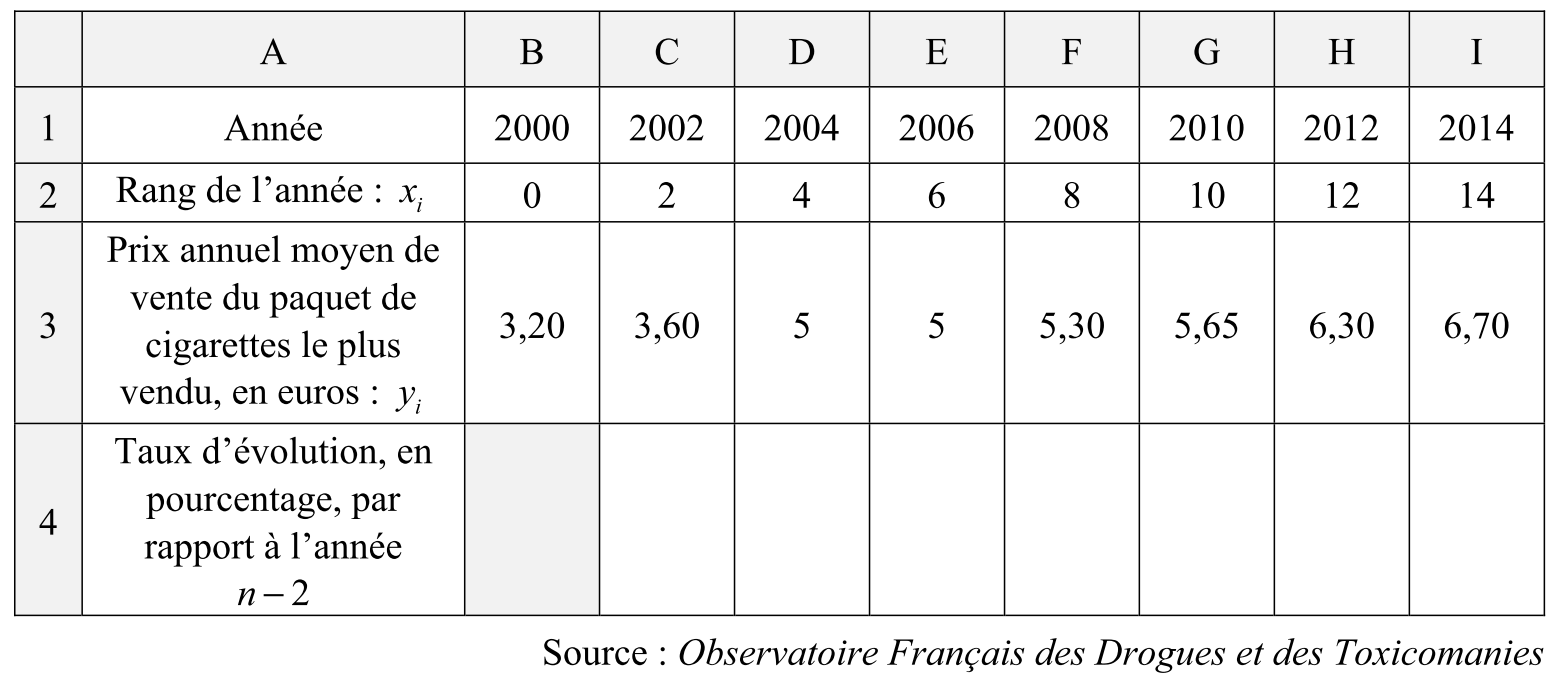
\includegraphics[scale=0.4]{img/tabac}
\end{center}

\subsection{(2 points)}

\begin{questions}
	\question[1] Un journaliste affirme que le prix entre 2000 et 2014 a augmenté de $50$ \%. L'affirmation est-elle vraie ou fausse ? Justifier.
	
	\question[1] La ligne 4 est au format pourcentage. Quelle formule peut-on saisir dans la cellule $C4$ et recopier vers la droite pour compléter la ligne 4 ?
\end{questions}

\subsection{(4 points)}

\begin{questions}
	\question[2]
	
		\begin{parts}
			\part[1] Sur la feuille de papier millimétré fournie et à rendre avec la copie, représenter le nuage de points de coordonnées $(x_i;y_i)$ dans un repère orthogonal en choisissant :
			\begin{itemize}
				\item 1cm pour 2 années en abscisse ;
				\item 1cm pour 1 euro en ordonnée.
			\end{itemize}
		
			\part[1] Calculer les coordonnées du point moyen $G$ du nuage de points, puis placer le point $G$ sur le graphique précédent. Arrondir les résultats à \num{0.01} près.
		\end{parts}
	
	\question[2] On admet que la droite $D$ d'équation $y=\num{0.24}x+\num{3.41}$ est un bon ajustement affine du nuage de points et que cet ajustement reste valable jusqu'en 2025.
		\begin{parts}
			\part[\half] Vérifier que le point $G$ appartient à la droite $D$.
			\part[\half] Tracer la droite $D$ sur le graphique précédent en indiquant les points utilisés.
			\part[\half] Selon cet ajustement, quel sera le prix moyen annuel d'un paquet de cigarettes en France en 2020 ?
			\part[\half] \'A partir de quelle année celui-ci dépassera-t-il les 10 euros ? Expliquer la démarche.
		\end{parts}
\end{questions}